\documentclass[a4paper]{article}
\usepackage[a4paper, margin=2cm]{geometry}
\usepackage{xgreek}
\usepackage{xltxtra}
\usepackage{unicode-math}
\usepackage{graphicx}
\usepackage{float}
%\usepackage{tocbibind}
\usepackage[pdfusetitle]{hyperref}
\graphicspath{{./images/}}
\setmainfont[Mapping=tex-text]{CMU Serif}
\setsansfont[Mapping=tex-text]{CMU Sans Serif}
\setmonofont{CMU Typewriter Text}
\usepackage{minted}
\usepackage{tocbibind}
\usepackage{caption}
\usepackage{subcaption}
\usepackage{svg}
\usepackage{fancyhdr}

\pagestyle{fancy}
\renewcommand{\headrulewidth}{0pt}
\fancyhf{}
\fancyfoot[C]{\thepage}
\fancyfoot[R]{\copyright\ \the\year\ Ανδρέας Στάμος - Κωνσταντίνος Πίκουλας}


\title{Τεχνική αναφορά\\\Large Πληροφοριακό σύστημα Δικτύου Σχολικών Βιβλιοθηκών\\\vspace{1em} \normalsize \url{https://github.com/andreasstamos/library-management-system}}
\author{Ανδρέας Στάμος - Κωνσταντίνος Πίκουλας}
\date{}

\hypersetup{
        pdfinfo={
            Title={Τεχνική Αναφορά - Πληροφοριακό σύστημα Δικτύου Σχολικών Βιβλιοθηκών},
            Author={Ανδρέας Στάμος - Κωνσταντίνος Πίκουλας}
        },
	colorlinks=true,
	linkcolor=blue,
        urlcolor=blue,
}

 
\begin{document}

\maketitle
\thispagestyle{fancy}

\tableofcontents

\section{Σχεδίαση εφαρμογής}

\begin{figure}[H]
\centering

\subcaptionbox{PostgreSQL}{\includesvg[height=0.1\textwidth]{images/postgresql_logo.svg}}
\hspace{1em}
\subcaptionbox{Flask}{\includesvg[height=0.1\textwidth]{images/flask_logo.svg}}
\hspace{1em}
\subcaptionbox{React}{\includesvg[height=0.1\textwidth]{images/react_logo.svg}}
\hspace{1em}
\subcaptionbox{Material UI}{\includesvg[height=0.1\textwidth]{images/mui_logo.svg}}
\caption{Web Development Stack}
\label{stack_logos}
\end{figure}

\par Η εφαρμογή σχεδιάστηκε σε stack: PostgreSQL, Flask, React, Material UI (υλοποίηση του Google Material Design σε React Components). (βλ και σχήμα \ref{stack_logos}).

\par Με χρήση του Flask αναπτύχθηκε \textbf{RESTful API} (δεν διατηρείται πουθενά state για τα sessions), ενώ με χρήση React αναπτύχθηκε Web εφαρμογή που τρέχει αποκλειστικά στον client (σερβίρονται αποκλειστικά τα στατικά αρχεία JavaScript της εφαρμογής) και που με HTTP Requests επικοινωνεί με το API.

\par Στο API τα requests έχουν την μορφή JSON, γίνονται με χρήση HTTP POST και γίνονται validate ότι έχουν την σωστή μορφή με χρήση ενός \textbf{JSONSchema} για κάθε διαφορετικό endpoint.

\par Σε περιβάλλον παραγωγής η επικοινωνία με το API γίνεται με HTTPS.

\section{Βάση δεδομένων}

\subsection{Διάγραμμα Οντοτήτων-Συσχετίσεων (Entity-Relationship Diagram)}

\par Αρχικά σχεδιάστηκε το σχήμα σε διάγραμμα οντοτήτων-συσχετίσεων (Entity-Relationship Diagram) όπως φαίνεται στην εικόνα \ref{er_diagram}.

\begin{figure}[H]
    \centering
    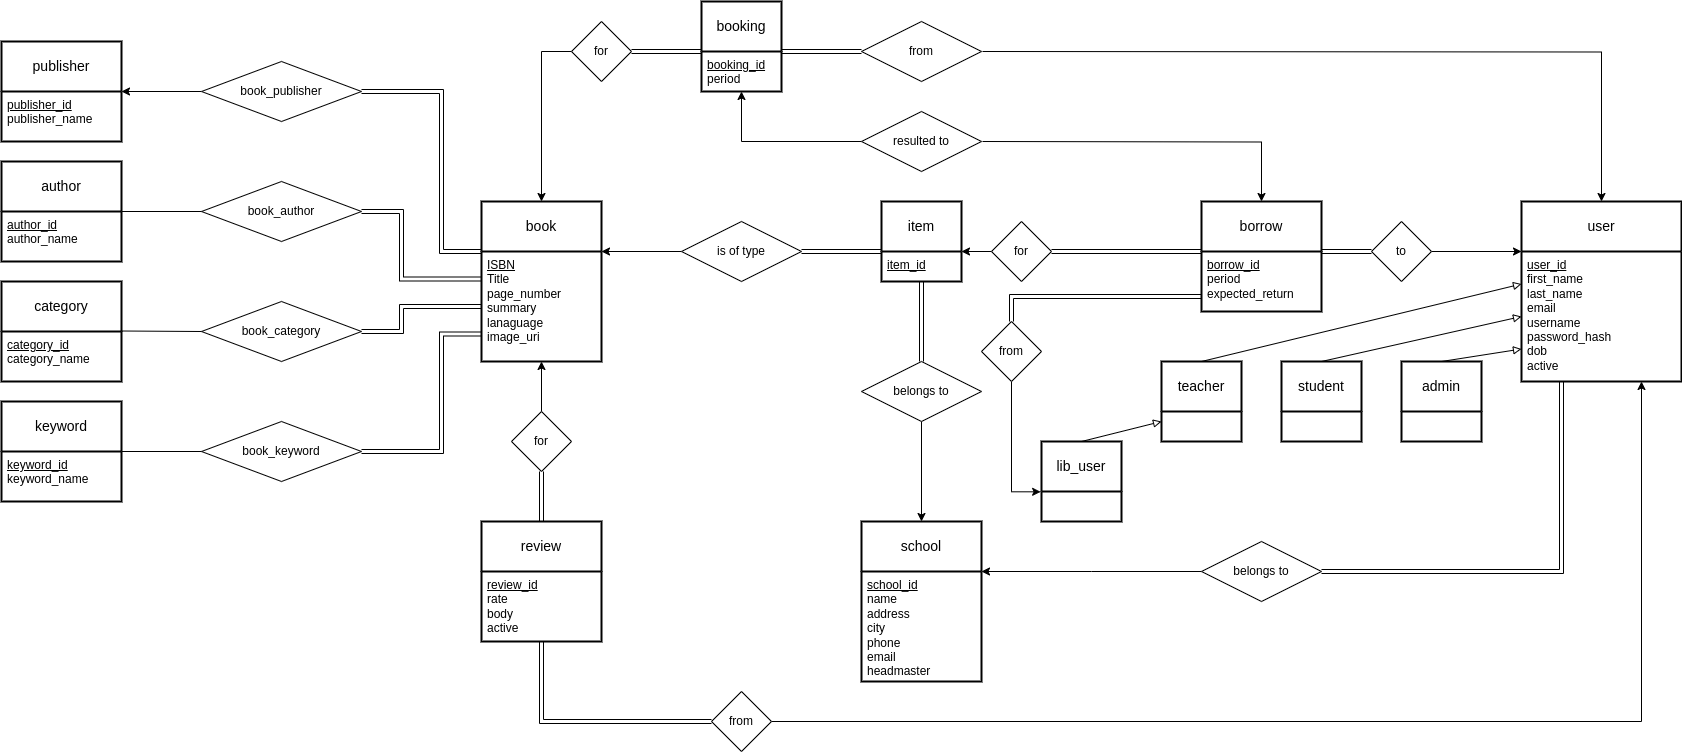
\includegraphics[width=\textwidth]{images/er.png}
    \caption{Διάγραμμα Οντοτήτων-Συσχετίσεων (Entity-Relationship Diagram)}
    \label{er_diagram}
\end{figure}

\subsection{Σχεσιακό σχήμα (Relational Schema)}

\par Στην συνέχεια σχεδιάστηκε με βάση αυτό το relational σχήμα της βάσης δεδομένων σχεδιάστηκε σύμφωνα με την \textbf{κανονική μορφή Boyce-Codd (BCNF)} (κάθε σύνολο attributes προκύπτει μόνο από υπερκλειδί), προκειμένου να μην υπάρχει πλεονασμός δεδομένων. Το DDL script για την κατασκευή της βάσης υπάρχει στο παράρτημα \ref{appendix_ddl} και το προκύπτον σχεσιακό διάγραμμα (relational diagram) φαίνεται στο σχήμα \ref{relational_diagram}.

\begin{figure}[H]
    \centering
    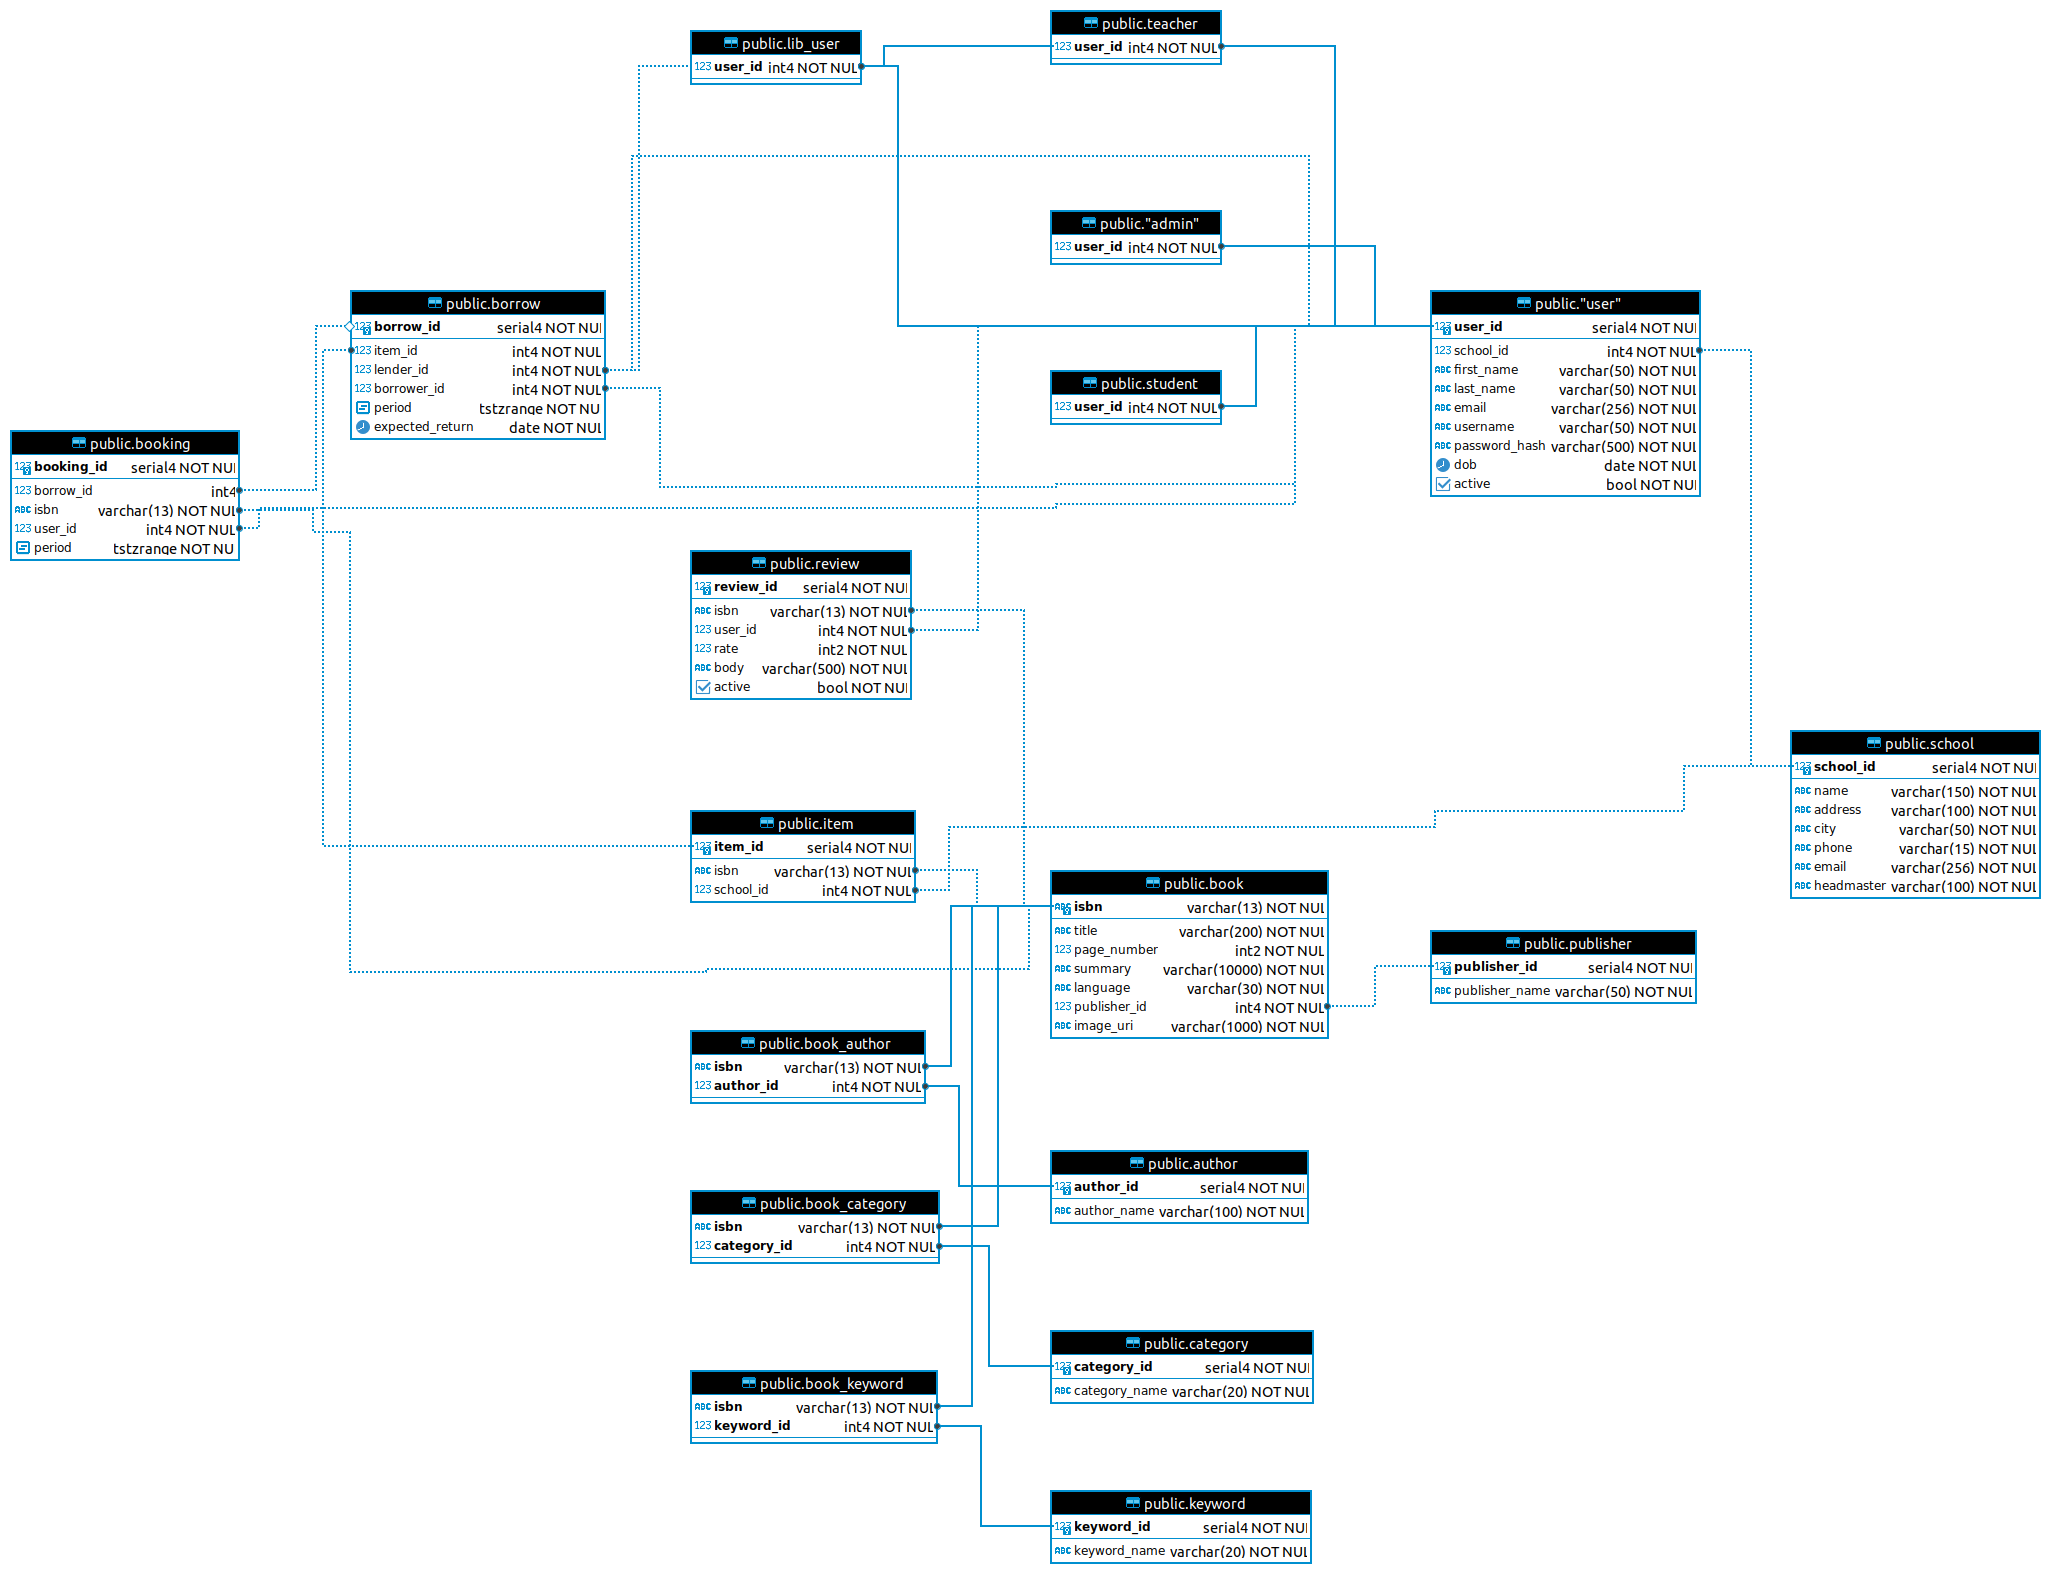
\includegraphics[width=\textwidth]{images/relational.png}
    \caption{Σχεσιακό Διάγραμμα (Relational Diagram)}
    \label{relational_diagram}
\end{figure}

\par Προκειμένου να διασφαλίσουμε την σωστή χρονολογική σειρά των δανεισμών (/των κρατήσεων), δηλαδή ότι μια δεδομένη χρονική στιγμή κάθε αντίτυπο είναι δανεισμένο σε έναν μόνο χρήστη (/κάθε χρήστης έχει μόνο μια κράτηση για ένα βιβλίο) χρησιμοποιήσαμε τον τύπο δεδομένου TSTZRANGE της PostgreSQL και με χρήση EXCLUDE επιβάλαμε τον περιορισμό ότι δύο tuples που αναφέρονται στο ίδιο αντίτυπο (/αντίστοιχα στο ίδιο βιβλίο και χρήστη για κρατήσεις) δεν θα πρέπει να έχουν χρονική επικάλυψη. Η PostgreSQL με χρήση GIST ευρετηρίου μπορεί να επιβάλλει αποδοτικά τον περιορισμό αυτό.

\par Η κατανομή ρόλων στους χρήστες αποτυπώθηκε στην βάση με χρήση Specialization στην ER σχεδίαση. Στο relational σχήμα αυτό μεταφράστηκε σε ξεχωριστούς πίνακες για κάθε ρόλο που απλά περιέχουν τα user\_id των χρηστών που κατέχουν τον αντίστοιχο ρόλο.

\subsection{Ευρετήρια}

\par Με δεδομένα τις ερωτήσεις που γίνονται στην βάση, δημιουργήσαμε και τα κατάλληλα ευρετήρια. Αξίζει να επισημανθεί ότι σε μερικά σημεία η αναζήτηση γίνεται σε ελέυθερο κείμενο, με χρήση των trigrams της PostgreSQL που υπολογίζουν μια μετρική similiarity μεταξύ συμβολοσειρών. Χρησιμοποιήθηκαν τα ειδικά ευρετήρια τύπου GIST για τους τελεστές των trigrams για τα συγκεκριμένα πεδία.

\par Επιπλέον αναφέρεται πως όπου επιβάλλεται στο σχήμα περιορισμός UNIQUE ούτως ή αλλώς δημιουργείται ευρετήριο για τα πεδία αυτά, οπότε δεν απαιτείται να δημιουργηθεί νέο αν αυτό απαιτηθεί για λόγους αναζήτησης.

\par Επισημαίνεται πως τα ευρετήρια έχουν σχεδιαστεί προσεγγιστικά με στόχο την βελτιστοποίηση της απόδοσης. Κατά την διάρκεια της ζωής της βάσης δεδομένων και σε βάθος χρόνου, θα πρέπει να μελετηθεί η συχνότητα εμφάνισης των διάφορων ερωτήματων και το κόστος υπολογισμού τους, προκειμένου να επαναξιολογηθούν τα απαιτούμενα ευρετήρια. Ενδέχεται σε μερικά σημεία, το κόστος συνεχούς ενημέρωσης του ευρετηρίου ενός πίνακα που ενημερώνεται συνεχώς να αποδειχθεί ότι δεν αξίζει για ένα ερώτημα που τελικά ερωτάται σπανίως.

\par Αναλυτικότερα, δημιουργήθηκαν ευρετήρια τύπου B+ tree στα:
\begin{itemize}
    \item publisher\_id του table book (χρήση στο φιλτράρισμα βιβλίων)
    \item email του table "user" (χρήση στο ``Ξέχασα τον κωδικό μου'')
    \item active του table "user" (ο χειριστής βιβλιοθήκης βλέπει τους inactive χρήστες, οι inactive χρήστες αναμένονται λίγοι)
    \item school\_id του table "user" (γίνεται φιλτράρισμα σε πολλά σημεία να βρίσκονται οι χρήστες ενός συγκεκριμένου σχολείου)
    \item isbn του table item (στην σελίδα ενός βιβλίου εμφανίζονται τα αντίτυπα ενός βιβλίου)
    \item ischool\_id του table item (σε πολλά ερωτήματα γίνεται ελέγχος ορθότητας-ασφάλειας πως ο χειριστής ενός σχολείου έχει δικαιώματα για πράξεις σε ένα συγκεκριμένο αντίτυπο)
    \item active του table review (ο χειριστής βιβλιοθήκης βλέπει τις inactive αξιολογήσεις, οι inactive αξιολογήσεις ανεμένονται λίγες)
    \item isbn του table review (στη σελίδα ενός βιβλίου εμφανίζονται οι αξιολογήσεις ενός βιβλίου, στην σελίδα όλων των βιβλίων εμφανίζονται μέσοι όροι αξιολογήσεων για όλα τα βιβλία)
    \item item\_id του table borrow (στην φόρμα Δανεισμού/Επιστροφής γίνεται έλεγχος αν ένα αντίτυπο είναι δανεισμένο ή όχι)
    \item borrower\_id του table borrow (ο χρήστης μπορεί να δει τους δανεισμούς του, επίσης ο χειριστής μπορεί να κάνει αναζήτηση δανεισμών ανά χρήστη)
    \item isbn του table booking (όταν γίνεται δανεισμός γίνεται ελέγχος για κρατήσεις στο ίδιο βίβλιο)
    \item user\_id του table booking (ο χρήστης μπορεί να δει τις κρατήσεις του, επίσης ο χειριστής μπορεί να κάνει αναζήτηση κρατήσεων ανά χρήστη)
\end{itemize}
\par Επιπρόσθετα ευρετήρια τύπου B+ tree δημιουργούνται και για όλα τα primary keys καθώς και για όλα τα πεδία όπου υπάρχει περιορισμός UNIQUE. Πολλά από αυτά τα ευρετήρια είναι και χρήσιμα για διάφορα ερωτήματα που γίνονται, όμως αυτό δεν απαιτείται να μελετηθεί εφόσον το UNIQUE ούτως ή αλλώς είναι αναγκαίο να υπάρχει για εξασφάλιση ορθότητας.

\par Επιπλέον δημιουργήθηκαν ευρετήρια τύπου GIST που εξυπηρετούν τα trigram operators στα:
\begin{itemize}
    \item author\_name του table author (γίνεται αναζήτηση του author\_name στο Autocomplete του search bar στα φίλτρα βιβλίων και στην εισαγωγή βιβλίου)
    \item publisher\_name του table publisher (γίνεται αναζήτηση του publisher\_name στο Autocomplete του search bar στα φίλτρα βιβλίων και στην εισαγωγή βιβλίου)
    \item category\_name του table category (γίνεται αναζήτηση του category\_name στο Autocomplete του search bar στα φίλτρα βιβλίων και στην εισαγωγή βιβλίου)
    \item keyword\_name του table keyword (γίνεται αναζήτηση του keyword\_name στο Autocomplete του search bar στα φίλτρα βιβλίων και στην εισαγωγή βιβλίου)
    \item συνδυασμό first\_name, last\_name του table "user" (γίνεται φιλτράρισμα βάσει ονοματεπώνυμου σε διάφορες σελίδες του χειριστή βιβλιοθήκης)
    \item title του table book (γίνεται αναζήτηση του title στην εμφάνιση λίστας βιβλίων, καθώς και στο Autocomplete του search bar στα φίλτρα βιβλίων).
\end{itemize}

\subsection{Mock data}
\label{mock_data}
\par Για τους σκοπούς ελέγχου της λειτουργίας του Συστήματος, κατασκευάστηκαν δεδομένα ελέγχου με χρήση της βιβλιοθήκης Faker της Python. Ενδεικτικά αναφέρεται ότι εισάγονται 5 σχολεία, 500 χρήστες, 1000 βιβλία, 10000 αντίτυπα, 10000 αξιολογήσεις, 5000 δανεισμοί και 1500 κρατήσεις.

\section{Αυθεντικοποίηση (Authentication) - Εξουσιοδότηση (Authorization)}

\subsection{Αυθεντικοποίηση (Authentication)}

\par Η αυθεντικοποίηση των χρηστών γίνεται με χρήση username, password όπου το password γίνεται hash με χρήση \textit{bcrypt} και κατόπιν salting. Το υπολογιστικά βαρύ bcrypt σε συνδυασμό με salting καθιστούν δύσκολη επίθεση bruteforce κατά των hash, ακόμα και αν γινόταν attack τύπου Rainbow Table.

\par Αφού αυθεντικοποιηθεί ο χρήστης, του χορηγείται ένα authentication token, υλοποιημένο ως JSON Web Token, ορισμένης χρονικής διάρκειας, που περιέχει πληροφορίες για το user\_id, το school\_id και τον ρόλο του χρήστη. Το token έχει expiration time 5 ωρών και έπειτα απαιτείται επανασύνδεση. Η παραχάραξη του token αποκλείεται καθώς περιέχει Ψηφιακή Υπογραφή του API. Το authentication token χορηγείται σε κάθε request στο API ως HTTP Authentication Header και από την εγκυρότητά του εξασφαλίζεται ότι ο χρήστης που στέλνει το request είναι αυθεντικοποιημένος.

\subsection{Εξουσιοδότηση (Authorization)}

\par Στην βάση δεδομένων έχουν δημιουργηθεί χωριστοί πίνακες για κάθε ρόλο, που περιέχουν τα user\_ids των χρηστών που διαθέτουν τον ρόλο αυτό. Όταν γίνει login, αφού γίνεται ελέγχος αυθεντικοποίησης, ελέγχεται αν ο χρήστης ανήκει σε κάποιον πίνακα και του απονέμεται ο αντίστοιχος ρόλος (δηλαδή ο αντίστοιχος ρόλος τοποθετείται ως role στο authentication token).

\par Σε επίπεδο API, το δικαίωμα ενός χρήστη για μια συγκεκριμένη πράξη ελέγχεται με βάση το role που λαμβάνεται στο authentication token μαζί με κάθε request.

\par Σε επίπεδο Web εφαρμογής, ελέγχεται σε κάθε route αν ο χρήστης διαθέτει το απαιτούμενο role πριν εμφανιστεί η σχετική σελίδα. Επισημαίνεται πως αυτό δεν προσφέρει πραγματική ασφάλεια, παρά μόνο εμφανίζει στον χρήστη τις σελίδες που μπορεί να έχει πρόσβαση. Αυτό διότι ούτως ή άλλως, ένας κακόβουλος χρήστης μπορεί να κάνει απευθείας requests στο API παρακάμπτοντας το Web App, και επίσης καθώς ο κώδικας της εφαρμογής εκτελείται πλήρως στον client, δηλαδή είναι πλήρως διαθέσιμος στον τελικό χρήστη, οπότε ένας κακόβουλος χρήστης θα μπορούσε απλά να αλλάξει τον κώδικα της εφαρμογής παρακάμπτοντας τους σχετικούς ελέγχους. (ακόμα και αν το κάνει αυτό το API δεν θα του δώσει δεδομένα).

\appendix

\section{Βιβλιοθήκες και Frameworks που χρησιμοποιήθηκαν}
\label{used_software}
\begin{enumerate}
    \item PostgreSQL
    \item Python
    \item Βιβλιοθήκες Python:
    \begin{enumerate}
        \item Flask (και flask\_cors, flask\_jwt\_extended)
        \item Psycopg2
        \item jsonschema
        \item bcrypt
        \item latex (βιβλιοθήκη της python για παραγωγή pdf αρχείου από LaTeX, χρησιμοποιείται για την δημιουργία κάρτας βιβλιοθήκης)
    \item TeX Live - LaTeX + package ``qrcode'' (για την δημιουργία κάρτας βιβλιοθήκης)
    \end{enumerate}   
    \item React
    \item React Router DOM
    \item Βιβλιοθήκες JavaScript:
    \begin{enumerate}
        \item Axios
        \item lodash
        \item jwt-decode
        \item dayjs
        \item file-saver
    \end{enumerate}
    \item Material UI (+ Material Icons)
\end{enumerate}

\section{DDL Script}
\label{appendix_ddl}
Το DDL Script που κατασκευάζει τους πίνακες τις βάσεις (και τα σχετικά ευρετήρια) βρίσκεται στο αποθετήριο GitHub στο path:
\mint{bash}|sql/schema.sql|
Επιπλέον ο διαδικτυακός υπερσύνδεσμος για το DDL Script απευθείας στο GitHub αποθετήριο είναι:\\
\url{https://github.com/andreasstamos/library-management-system/blob/master/sql/schema.sql}

\inputminted[breaklines,linenos]{sql}{../../sql/schema.sql}

\section{DML Script}

\par Το DML Script που εισάγει τα Mock Data στην βάση, τα οποία δημιουργήθηκαν σύμφωνα με την διαδικασία που αναφέρθηκε στην ενότητα \ref{mock_data} βρίσκεται στο αποθετήριο GitHub στο path:
\mint{bash}|fake_data/fake_data.sql|
Επιπλέον ο διαδικτυακός υπερσύνδεσμος για το DDL Script απευθείας στο GitHub αποθετήριο είναι:\\
\url{https://github.com/andreasstamos/library-management-system/blob/master/fake_data/fake_data.sql}

\par Το αρχείο αυτό δημιουργείται αυτόματα αν (αφού εγκαταστήσετε την βιβλιοθήκη Faker) τρέξετε την εντολή:
\mint{bash}|python3 create.py|
Η γεννήτρια τυχαίων αριθμών έχει ρυθμιστεί με σταθερό seed προκειμένου τα αποτέλεσματα να είναι ντετερμινιστικά.

\section{Οδηγίες Εγκατάστασης}

\subsection{Βάση Δεδομένων}
\label{install_db}
\par Αρχικά πρέπει να εγκαταστήσετε την PostgreSQL (έκδοση 14+), να δημιουργήσετε μια βάση δεδομένων (πχ. με χρήση της εντολής \mintinline{bash}{createdb}) και να δημιουργήσετε επιπλέον έναν χρήστη στην βάση δεδομένων, ο οποίος θα έχει δικαίωμα να δημιουργεί και κάνει drop πίνακες, καθώς επίσης και θα έχει δικαίωμα εγγραφής/ανάγνωσης σε αυτούς. (προκειμένου το backup/restore να λειτουργεί ο χρήστης θα πρέπει να έχει δικαιώματα να κάνει DROP τους πίνακες που θα κατασκευαστούν, καθώς και να τους δημιουργήσει).
\par Με χρήστη του συστήματος σας PostgresSQL που έχει δικαιώματα για αυτό, πρέπει έπειτα να εκτέλεσετε τα αρχεία \mintinline{bash}{sql/schema.sql} και \mintinline{bash}{sql/borrow.sql} που αντίστοιχα κατασκευάζουν τους πίνακες με τα ευρετήρια και εισάγουν μερικές απαραίτητες SQL Functions στην βάση.

\par Οι λεπτομέρειες εγκατάστασης της βάσης δεδομένων, ανάλογα πάντα και με το λειτουργικό σας σύστημα ξεφεύγουν του παρόντος οδηγού. Σας παραπέμπουμε στην επίσημη ιστοσελίδα της PostgreSQL για αναλυτικότερες οδηγίες.

\subsection{Backend (API)}

\par Αρχικά πρέπει να εγκαταστήσετε την python3. Επίσης πρέπει να εγκαταστήσετε το pdflatex του TexLive καθώς επίσης και να εξασφαλίσετε ότι το package qrcode του LaTex είναι εγκατεστημένο. Προτείνουμε την χρήση του Package Manager του λειτουργικού σας συστήματος αν δουλεύετε σε υπολογιστικό σύστημα Linux (για το LaTeX και το package του qrcode σε περιβάλλον Ubuntu/Debian τα πακέτα texlive-latex-recommended και texlive-pictures επαρκούν), διαφορετικά ακολουθήστε τις οδηγίες που προτείνονται στις επίσημες ιστοσελίδες των λογισμικών για την εγκατάστασή τους στο σύστημά σας.

\par Προτείνουμε η εγκατάσταση των βιβλιοθηκών Python να γίνει σε Virtual Environment και με χρήση pip3 για αποφυγή προβλημάτων συμβατότητας. Αν επιθυμείτε να εγκαταστήσετε με διαφορετικό τρόπο τις προαπαιτούμενες βιβλιοθήκες ή το σύστημα σας δεν υποστηρίζει Python Virtual Environment και pip3, σας παραπέμπουμε στο παράρτημα \ref{used_software} καθώς και στο αρχείο \mintinline{bash}{backend/requirements.txt} για τις σχετικές απαιτήσεις.

\par Το λειτουργικό σας σύστημα ενδεχομένως να έχει προεγκατεστήμενο το Python Virtual Envirionment. Διαφορετικά εγκαταστήστε τα με την εντολή: \mintinline{bash}{pip3 install virtualenv}

\par Ακολουθήστε τα παρακάτω βήματα σε ένα τερματικό:
\begin{enumerate}
    \item Εισέλθετε στον φάκελο του backend.
        \mint{bash}|cd backend|
    \item Με τον αγαπημένο σας editor (πχ. vi) επεξεργαστείτε το αρχείο \mintinline{bash}{config.py}.
        \par Θέστε στις μεταβλητές DB\_HOST, DB\_PORT, DB\_NAME, DB\_USER, DB\_PASSWORD αντίστοιχα στην IP διεύθυνση του server του σύστηματος PostgrsSQL σας, στο TCP port του, στο όνομα της βάσης δεδομένων που θα χρησιμοποιήσει το παρόν σύστημα, στο όνομα χρήστη του σύστηματος PostgreSQL σας που θα χρησιμοποιήσει το παρόν σύστημα καθώς και στο password του. Αν δεν γνωρίζετε ένα ή περισσότερα από τα στοιχεία αυτά, σας παραπέμπουμε στην διαδικασία του παραρτήματος \ref{install_db} και στην επίσημη ιστοσελίδα της PostgreSQL για περισσότερες πληροφορίες.
        \parΕπίσης θέστε στην μεταβλητή JWT\_SECRET\_KEY μια κατάλληλη κρυπτογραφικά τυχαία τιμή, η οποία θα χρησιμοποιηθεί για την Ψηφιακή Υπογραφή του authentication token που θα αποστέλλει το API όταν αυθεντικοποείται κάποιος χρήστης.
        \par Μην κοινοποιήσετε πουθένα την τιμή αυτή, όπως φυσικά και κανένα από τα υπόλοιπα στοιχεία.
    \item Δημιουργήστε το Python Virtual Environment.
        \mint{bash}|python3 -m venv venv|
    \item Ενεργοποιήστε στο τερματικό που βρίσκεστε το Python Virtual Environment.
        \mint{bash}|source venv/bin/activate|
    \item Εγκαταστήστε τις προαπαιτούμενες βιβλιοθήκες.
        \mint{bash}|pip3 install -r requirements.txt|
    \item Εκτελέστε το backend με χρήση του Development Server του Flask:
        \mint{bash}|python3 run.py|
\end{enumerate}

\textbf{ΠΡΟΣΟΧΗ/Disclaimer:} Οι παραπάνω οδηγίες θα οδηγήσουν στο να τρέχει το backend στον τοπικό υπολογιστή με τον Development Server του Flask θέτοντας πιθανώς τον υπολογιστή σας σε κινδύνους ασφαλείας. Αυτός προφανώς αντιπροτείνεται για χρήση σε περιβάλλον παραγωγής. Την εγκατάσταση σε περιβάλλον παραγωγής θα πρέπει να αναλάβουν πεπειραμένοι χρήστες εγκαθιστώντας και ρυθμίζοντας ενδεικτικά αλλά όχι αποκλειστικά reverse proxy (πχ. nginx), ssl πιστοποιητικά, firewalls κλπ. Καμία ευθύνη δεν φέρουν οι developers σε καμία περίπτωση για πιθανά προβλήματα ασφαλείας.

\subsection{Web Application}

\par Αρχικά πρέπει να εγκαταστήσετε την python3. Προτείνουμε την χρήση του Package Manager του λειτουργικού σας συστήματος αν δουλεύετε σε υπολογιστικό σύστημα Linux, διαφορετικά ακολουθήστε τις οδηγίες που προτείνονται στις ιστοσελίδες τους για την εγκατάστασή τους στο σύστημα σας.

\par Αφού εισέλθετε στον φάκελο του Web Application με την εντολή:
\mint{bash}|cd client|
εγκαταστήσετε εύκολα τα προαπαιτούμενα για το Web Application με την εντολή:
\mint{bash}|npm i|

\par Μπορείτε να τρέξετε στον τοπικό υπολογιστή έναν Development Server που να σερβίρει την Web Application. Αυτός προφανώς αντιπροτείνεται για περιβάλλον παραγωγής. Ισχύει το ίδιο Disclaimer και η αποποίηση ευθύνης που αναφέρθηκε παραπάνω για το backend. Προκειμένου να τρέξετε τον Develpment Server τρέξτε την εντολή:
\mint{bash}|npm start|

\par Αν επιθυμείτε να εγκαταστήσετε την Web Application σε έναν server με σκοπό την χρήση σε περιβάλλον παραγωγής και μόνο εφόσον είστε πεπειραμένος χρήστης και πάντα αποκλειστικά με δική σας ευθύνη, μπορείτε να κάνετε compile την εφαρμογή με χρήση της εντολής:
\mint{bash}|npm build|
Στην συνέχεια τα περιεχόμενα του φακέλου \mintinline{bash}{build/} θα πρέπει να σερβιριστούν ως στατικά αρχεία από τον αγαπημένο σας Διακομιστή Ιστού (πχ. Nginx/Apache) ή από το αγαπημένο σας Hosting Provider.

\end{document}
